\documentclass[]{article}
\usepackage{lmodern}
\usepackage{amssymb,amsmath}
\usepackage{ifxetex,ifluatex}
\usepackage{fixltx2e} % provides \textsubscript
\ifnum 0\ifxetex 1\fi\ifluatex 1\fi=0 % if pdftex
  \usepackage[T1]{fontenc}
  \usepackage[utf8]{inputenc}
\else % if luatex or xelatex
  \ifxetex
    \usepackage{mathspec}
  \else
    \usepackage{fontspec}
  \fi
  \defaultfontfeatures{Ligatures=TeX,Scale=MatchLowercase}
\fi
% use upquote if available, for straight quotes in verbatim environments
\IfFileExists{upquote.sty}{\usepackage{upquote}}{}
% use microtype if available
\IfFileExists{microtype.sty}{%
\usepackage{microtype}
\UseMicrotypeSet[protrusion]{basicmath} % disable protrusion for tt fonts
}{}
\usepackage[margin=1in]{geometry}
\usepackage{hyperref}
\hypersetup{unicode=true,
            pdftitle={Supplementary Information, Usage frequency and lexical class determine the evolution of kinship terms in Indo-European},
            pdfauthor={Rácz, Passmore, Sheard, and Jordan},
            pdfborder={0 0 0},
            breaklinks=true}
\urlstyle{same}  % don't use monospace font for urls
\usepackage{color}
\usepackage{fancyvrb}
\newcommand{\VerbBar}{|}
\newcommand{\VERB}{\Verb[commandchars=\\\{\}]}
\DefineVerbatimEnvironment{Highlighting}{Verbatim}{commandchars=\\\{\}}
% Add ',fontsize=\small' for more characters per line
\usepackage{framed}
\definecolor{shadecolor}{RGB}{248,248,248}
\newenvironment{Shaded}{\begin{snugshade}}{\end{snugshade}}
\newcommand{\KeywordTok}[1]{\textcolor[rgb]{0.13,0.29,0.53}{\textbf{#1}}}
\newcommand{\DataTypeTok}[1]{\textcolor[rgb]{0.13,0.29,0.53}{#1}}
\newcommand{\DecValTok}[1]{\textcolor[rgb]{0.00,0.00,0.81}{#1}}
\newcommand{\BaseNTok}[1]{\textcolor[rgb]{0.00,0.00,0.81}{#1}}
\newcommand{\FloatTok}[1]{\textcolor[rgb]{0.00,0.00,0.81}{#1}}
\newcommand{\ConstantTok}[1]{\textcolor[rgb]{0.00,0.00,0.00}{#1}}
\newcommand{\CharTok}[1]{\textcolor[rgb]{0.31,0.60,0.02}{#1}}
\newcommand{\SpecialCharTok}[1]{\textcolor[rgb]{0.00,0.00,0.00}{#1}}
\newcommand{\StringTok}[1]{\textcolor[rgb]{0.31,0.60,0.02}{#1}}
\newcommand{\VerbatimStringTok}[1]{\textcolor[rgb]{0.31,0.60,0.02}{#1}}
\newcommand{\SpecialStringTok}[1]{\textcolor[rgb]{0.31,0.60,0.02}{#1}}
\newcommand{\ImportTok}[1]{#1}
\newcommand{\CommentTok}[1]{\textcolor[rgb]{0.56,0.35,0.01}{\textit{#1}}}
\newcommand{\DocumentationTok}[1]{\textcolor[rgb]{0.56,0.35,0.01}{\textbf{\textit{#1}}}}
\newcommand{\AnnotationTok}[1]{\textcolor[rgb]{0.56,0.35,0.01}{\textbf{\textit{#1}}}}
\newcommand{\CommentVarTok}[1]{\textcolor[rgb]{0.56,0.35,0.01}{\textbf{\textit{#1}}}}
\newcommand{\OtherTok}[1]{\textcolor[rgb]{0.56,0.35,0.01}{#1}}
\newcommand{\FunctionTok}[1]{\textcolor[rgb]{0.00,0.00,0.00}{#1}}
\newcommand{\VariableTok}[1]{\textcolor[rgb]{0.00,0.00,0.00}{#1}}
\newcommand{\ControlFlowTok}[1]{\textcolor[rgb]{0.13,0.29,0.53}{\textbf{#1}}}
\newcommand{\OperatorTok}[1]{\textcolor[rgb]{0.81,0.36,0.00}{\textbf{#1}}}
\newcommand{\BuiltInTok}[1]{#1}
\newcommand{\ExtensionTok}[1]{#1}
\newcommand{\PreprocessorTok}[1]{\textcolor[rgb]{0.56,0.35,0.01}{\textit{#1}}}
\newcommand{\AttributeTok}[1]{\textcolor[rgb]{0.77,0.63,0.00}{#1}}
\newcommand{\RegionMarkerTok}[1]{#1}
\newcommand{\InformationTok}[1]{\textcolor[rgb]{0.56,0.35,0.01}{\textbf{\textit{#1}}}}
\newcommand{\WarningTok}[1]{\textcolor[rgb]{0.56,0.35,0.01}{\textbf{\textit{#1}}}}
\newcommand{\AlertTok}[1]{\textcolor[rgb]{0.94,0.16,0.16}{#1}}
\newcommand{\ErrorTok}[1]{\textcolor[rgb]{0.64,0.00,0.00}{\textbf{#1}}}
\newcommand{\NormalTok}[1]{#1}
\usepackage{graphicx,grffile}
\makeatletter
\def\maxwidth{\ifdim\Gin@nat@width>\linewidth\linewidth\else\Gin@nat@width\fi}
\def\maxheight{\ifdim\Gin@nat@height>\textheight\textheight\else\Gin@nat@height\fi}
\makeatother
% Scale images if necessary, so that they will not overflow the page
% margins by default, and it is still possible to overwrite the defaults
% using explicit options in \includegraphics[width, height, ...]{}
\setkeys{Gin}{width=\maxwidth,height=\maxheight,keepaspectratio}
\IfFileExists{parskip.sty}{%
\usepackage{parskip}
}{% else
\setlength{\parindent}{0pt}
\setlength{\parskip}{6pt plus 2pt minus 1pt}
}
\setlength{\emergencystretch}{3em}  % prevent overfull lines
\providecommand{\tightlist}{%
  \setlength{\itemsep}{0pt}\setlength{\parskip}{0pt}}
\setcounter{secnumdepth}{0}
% Redefines (sub)paragraphs to behave more like sections
\ifx\paragraph\undefined\else
\let\oldparagraph\paragraph
\renewcommand{\paragraph}[1]{\oldparagraph{#1}\mbox{}}
\fi
\ifx\subparagraph\undefined\else
\let\oldsubparagraph\subparagraph
\renewcommand{\subparagraph}[1]{\oldsubparagraph{#1}\mbox{}}
\fi

%%% Use protect on footnotes to avoid problems with footnotes in titles
\let\rmarkdownfootnote\footnote%
\def\footnote{\protect\rmarkdownfootnote}

%%% Change title format to be more compact
\usepackage{titling}

% Create subtitle command for use in maketitle
\providecommand{\subtitle}[1]{
  \posttitle{
    \begin{center}\large#1\end{center}
    }
}

\setlength{\droptitle}{-2em}

  \title{Supplementary Information, Usage frequency and lexical class determine
the evolution of kinship terms in Indo-European}
    \pretitle{\vspace{\droptitle}\centering\huge}
  \posttitle{\par}
    \author{Rácz, Passmore, Sheard, and Jordan}
    \preauthor{\centering\large\emph}
  \postauthor{\par}
    \date{}
    \predate{}\postdate{}
  
\usepackage{booktabs}
\usepackage{longtable}
\usepackage{array}
\usepackage{multirow}
\usepackage{wrapfig}
\usepackage{float}
\usepackage{colortbl}
\usepackage{pdflscape}
\usepackage{tabu}
\usepackage{threeparttable}
\usepackage{threeparttablex}
\usepackage[normalem]{ulem}
\usepackage{makecell}
\usepackage{xcolor}

\begin{document}
\maketitle

{
\setcounter{tocdepth}{2}
\tableofcontents
}
\section{Kinship data}\label{kinship-data}

We collected kin terms from 45 languages for the following relations: B,
D, F, M, MB, MZ, MZD, MZS, S, Z, collected from a combination of native
speakers, ethnographies, and dictionaries in our
\href{https://excd.org/research-activities/kinbank/}{`Kinbank'
database}. Initially, the analyses used a broader set of kinship terms
(e.g.~FB, FZ), however we restricted the sample to form a comparable set
of word frequencies. This is because most Indo-European languages do not
have separate terms for e.g.~MZD and MBD and separate terms for e.g.~BW
are exceedingly rare (both across languages as types and within
languages as token). We have not included \emph{husband} and
\emph{wife}, because these are often synonymous with \emph{man} and
\emph{woman}, respectively.

Frequency data were collected from 34 corpora in 21 languages in three
corpus types: spoken, written, and web-crawled. The list of corpora is
in Table 1 below.

Table S1: Source of frequency data (source of words is Kinbank)

Language

Corpus name

Reference

Albanian

Albanian NC

(Morozova М 2015)

Bulgarian

Bulgarian NC

(Koeva, Blagoeva, and Kolkovska 2010)

Bulgarian

Bulgarian Web 2012 (bgTenTen12)

(Kilgarriff et al. 2014)

Catalan

Catalan Web 2014 (caTenTen14)

(Kilgarriff et al. 2014)

English

CELEX

(Baayen, Piepenbrock, and H 1993)

German

CELEX

(Baayen, Piepenbrock, and H 1993)

Spanish

CoE

(Moreno-Sandoval et al. 2005)

Portuguese

CoP

(Craveiro, Macedo, and Madeira 2012)

Italian

CORIS

(Favretti, Tamburini, and De Santis 2002)

Czech

Czech Web 2012 (czTenTen12 v8)

(Kilgarriff et al. 2014)

Danish

Danish Web 2014 (daTenTen14)

(Kilgarriff et al. 2014)

Dutch

Dutch Instituut voor Nederlandse Lexicologie text corpora (written)
Corpus Gesproken Nederlands (spoken)

(Kruyt and others 1997)

Dutch

Dutch Instituut voor Nederlandse Lexicologie text corpora (written)
Corpus Gesproken Nederlands (spoken)

(Van Eerten 2007)

Dutch

Dutch Web 2014 (nlTenTen14)

(Kilgarriff et al. 2014)

French

French Web 2012 (frTenTen12)

(Kilgarriff et al. 2014)

German

German Web 2013 (deTenTen13)

(Kilgarriff et al. 2014)

Greek

Greek Web 2014 (elTenTen14)

(Kilgarriff et al. 2014)

Croatian

hrWaC

(Kilgarriff et al. 2014)

Italian

Italian Web 2010 (itTenTen)

(Kilgarriff et al. 2014)

French

lexique corpus

(New et al. 2001)

Norwegian

Norwegian Web 2015 (noTenTen15) Bokmal and Nynorsk

(Kilgarriff et al. 2014)

Polish

Polish NC written PELCRA spoken

(Przepiórkowski et al. 2008)

Polish

Polish NC written PELCRA spoken

(Przepiórkowski et al. 2010)

Polish

Polish Web 2012 (plTenTen12)

(Kilgarriff et al. 2014)

Portuguese

Portuguese Web 2011 (ptTenTen11, Freeling v3)

(Kilgarriff et al. 2014)

English

pukWaC (ukWaC parsed with MaltParser)

(Kilgarriff et al. 2014)

Romanian

Romanian Web (roWaC)

(Kilgarriff et al. 2014)

Romanian

ROMBAC

(Ion et al. 2012)

Russian

Russian NC via Leeds

(Lyashevskaya and Sharov 2009)

Russian

Russian Web 2011 (ruTenTen11)

(Kilgarriff et al. 2014)

Serbian

scWaC

(Kilgarriff et al. 2014)

Spanish

Spanish Web 2011 (esTenTen11, Eu + Am, Freeling v4)

(Kilgarriff et al. 2014)

Swedish

SUC

(Gustafson-Capková and Hartmann 2006)

Swedish

Swedish Web 2014 (svTenTen14)

(Kilgarriff et al. 2014)

Icelandic

textasafn

(Úlfarsdóttir and Bjarnadóttir 2017)

Czech

UCNK:SYN2015 (written) ORAL2013 (spoken)

(Čermák 1997)

Czech

UCNK:SYN2015 (written) ORAL2013 (spoken)

(Benešová, Kren, and Waclawicová 2013)

The analysis uses one term per language per kinterm. If it arises that a
langauge has multiple words for a particular kinterm, we use which ever
was more frequent in the corpus data. In the case where a language has
multiple words for a single kinterm, and we do not have access to
frequency data, we rely on expert judgement to select a term.

\subsection{Supplementary data table}\label{supplementary-data-table}

See the supplementary data csv file for the raw data used in this study.

\paragraph{Column description:}\label{column-description}

Table S2: Supplementary table column descriptions

Column name

Description

meaning

Code used for kinterm, see TS1 for a description

language

Common name for each language

word

Words used in the analysis

lingpy.cognate

Cognates as determined by lingpy, used as a first pass

expert.cognate

Cognates reviewed and corrected by expert reviewers, used in analysis

word.count

Frequency of each term in the given corpus

corpora.size

Total size of the corpus

corpora.type

Type of corpus used (either web, written, or spoken)

corpus

Name of the corpus

states

States

taxa

Taxa label in phylogeny

glottocode

Glottocode

source.ids

Standard deviation for the global rate of replacement

mean.roc

Mean global rate of replacement

sd.roc

Source of term (see source SM)

\subsection{Data summary}\label{data-summary}

We estimate rate of replacement and compare it with frequency of use for
ten types of kin relations. Here we use MB, MZ, MZS, and MZD as
shorthand for broader terms (uncle, aunt, male cousin, and female
cousin, respectively). This is because commonly used terms in this set
of languages do not distinguish terms according to the parent's gender.

Below is a table indicating the shorthand used for each kinterm, the
number of languages for which we have data, and the number of states (or
cognates) for that term.

We collected terms for a superset of the languages from which frequency
data is available in order to have a more robust estimate of rate of
replacement for each term.

Table S3: Each kinterm used, with counts for the number of languages we
have data for and the number of cognates across our sample

Kinterm

Description

No. languages

States

F

Father

45

7

M

Mother

45

5

S

Son

43

7

D

Daughter

43

10

B

Brother

45

9

Z

Sister

44

6

MB

Mother's brother (uncle)

39

7

MZ

Mother's sister (aunt)

39

10

MZS

Mother's sister's daughter (female cousin)

31

11

MZD

Mother's sisters son (male cousin)

31

11

\subsection{Frequency data}\label{frequency-data}

Below are bar graphs of term frequency by langauge, across corpora types
(web, written, or spoken).

\begin{center}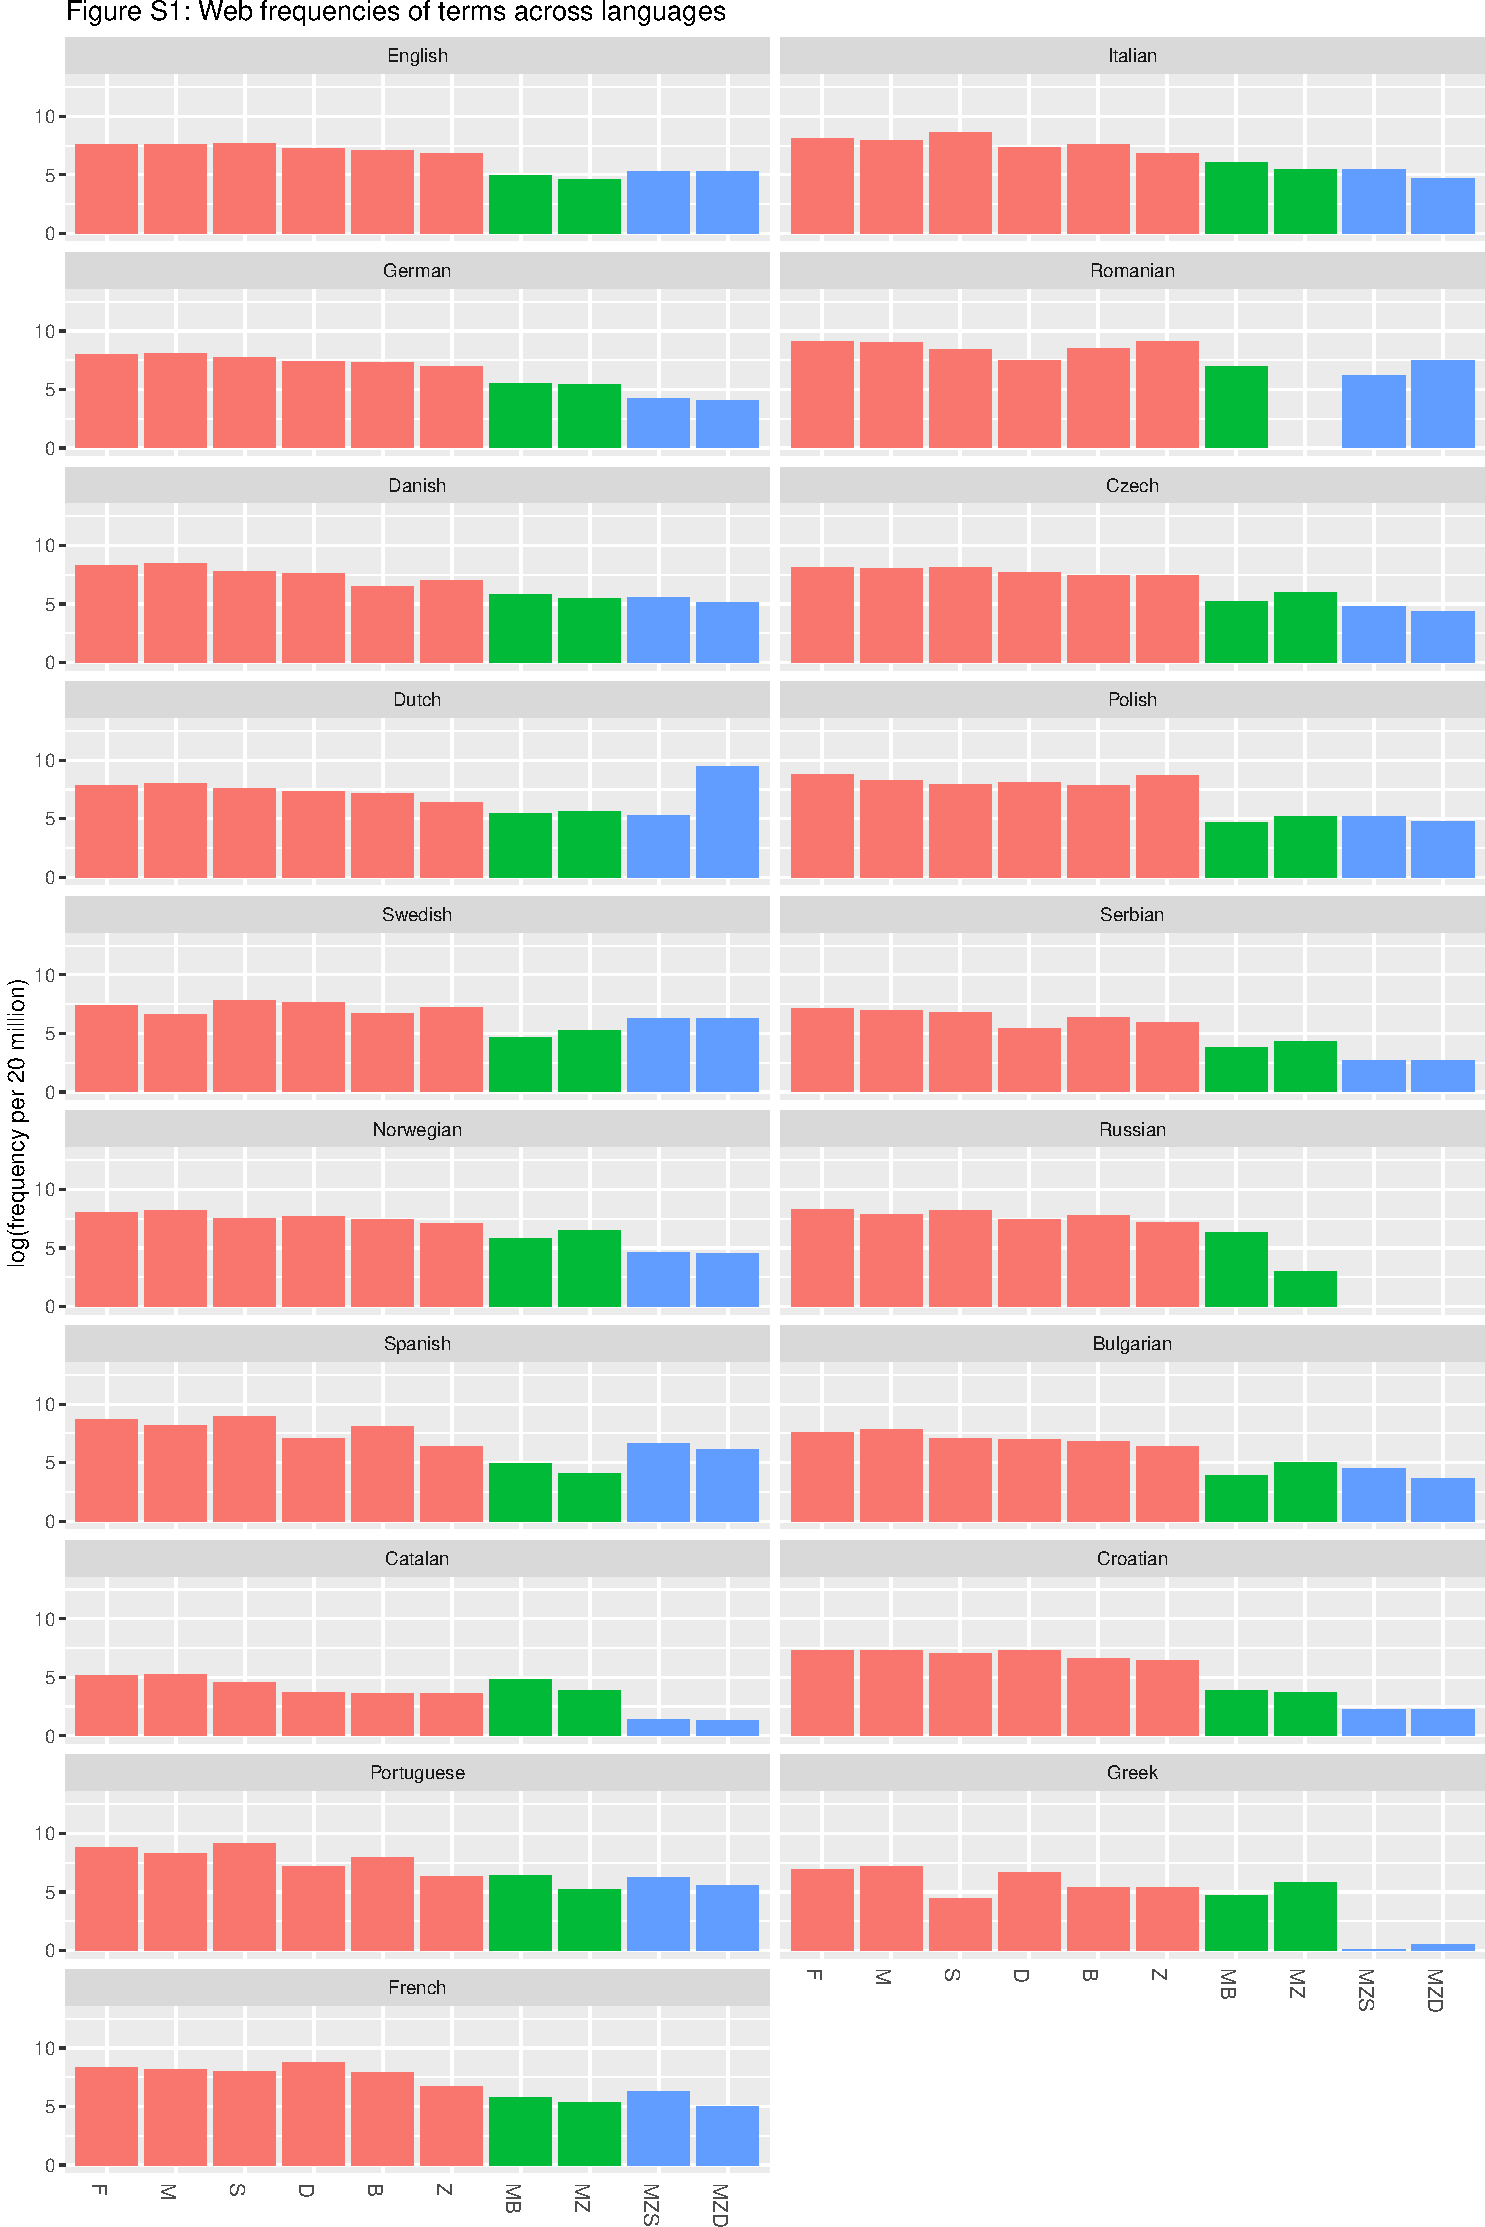
\includegraphics{figures/unnamed-chunk-6-1} \end{center}

\begin{center}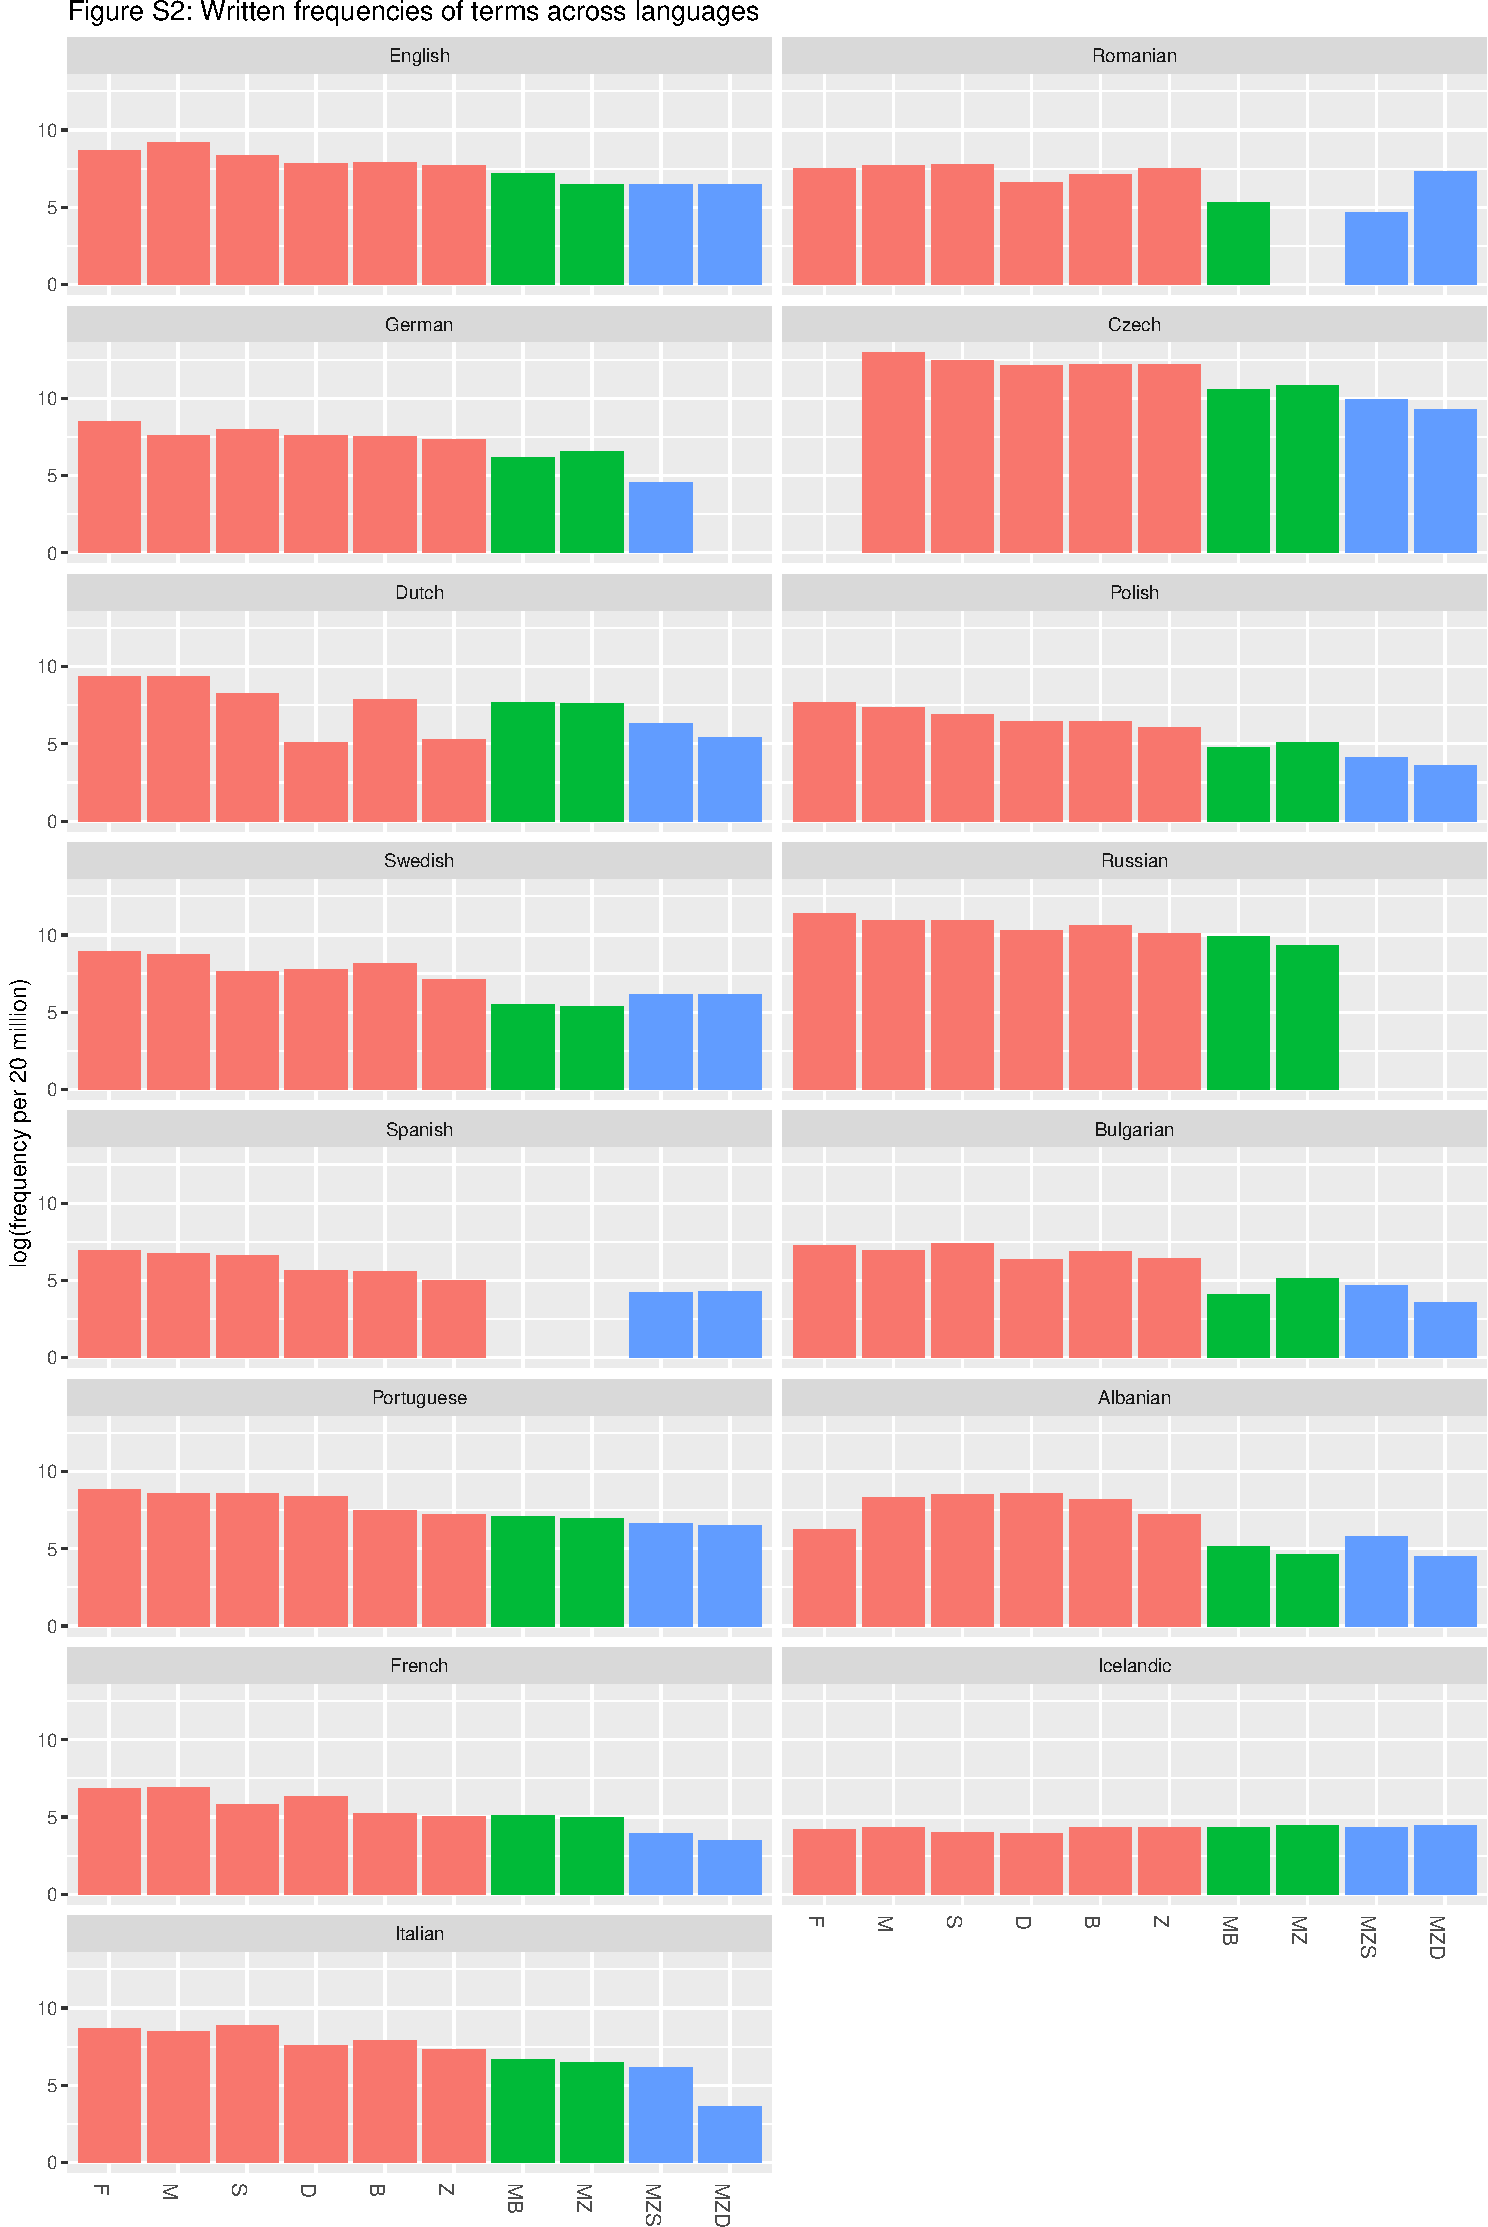
\includegraphics{figures/unnamed-chunk-6-2} \end{center}

\begin{center}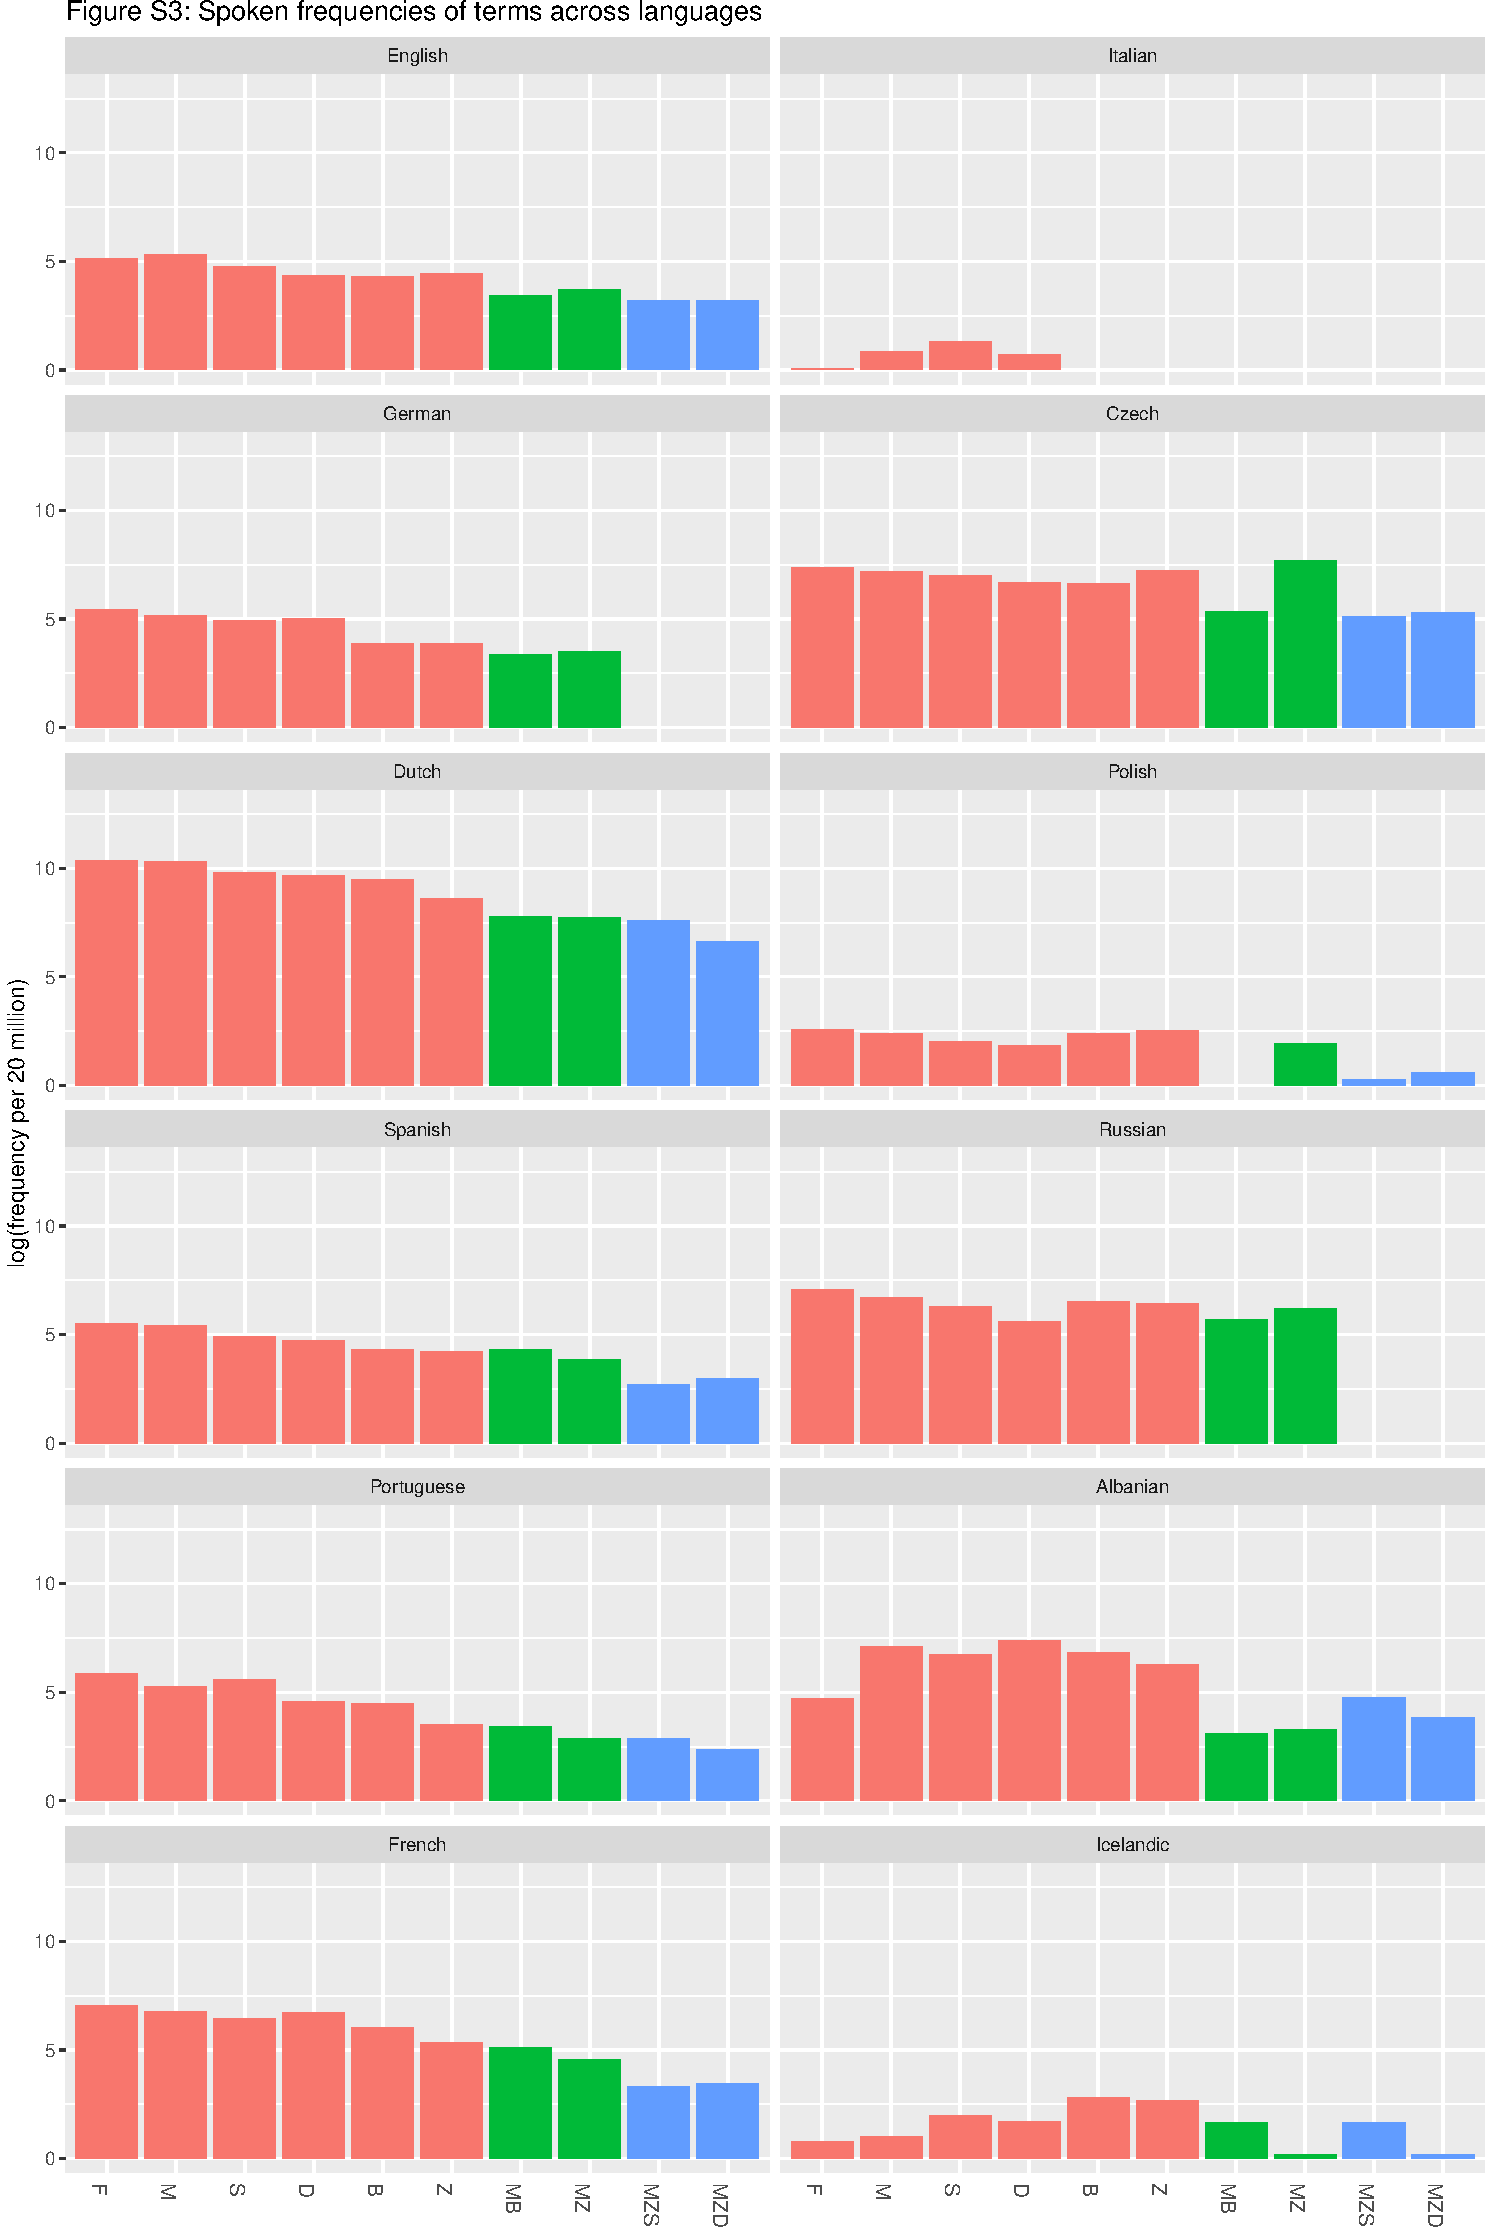
\includegraphics{figures/unnamed-chunk-6-3} \end{center}

\section{Cognate data}\label{cognate-data}

We generated cognate classes using the Indo-European Etymological
Dictionary (Buck 2008), LingPy (List, Greenhill, and Forkel 2018), and a
panel of volunteer experts, recruited on Linguist List (all faults
remain ours). All terms were automatically transcribed into the Speech
Assessment Methods Phonetic Alphabet (SAMPA) through LingPy's
\texttt{uni2sampa} function. Cognates were automatically allocated using
LingPy's \texttt{cluster} function. Using the cognate-coded Swadesh list
(subset to those languages for which we also have kinterms), we tested
the appropriateness of edit distance, SCA, and turchin algorithms,
alongside Phonemic and Phonetic transcriptions for cognate detection in
our data, following the code examples from
\href{http://lingpy.org/examples.html}{Lingpy.org}. The F-score was
highest for the edit-distance algorithm with a 0.4 threshold (see table
S4) (List, Greenhill, and Forkel 2018). We then manually adjusted the
results, followed by expert review which resulted in minor changes.
Automatic decisions and the corrections are available in the
supplementary data file.

Table S4: Precision, recall, \& F-score for various LingPy cognate
detection algorithms and their threshold settings.

transcription

threshold

method

precision

recall

fscore

Phonemic

0.4

edit

0.7792

0.4238

0.5490

Phonemic

0.6

edit

0.6259

0.4247

0.5060

Phonemic

0.4

turchin

0.5152

0.4271

0.4670

Phonemic

0.6

turchin

0.5152

0.4271

0.4670

Phonetic

0.4

edit

0.8434

0.3194

0.4634

Phonemic

0.4

sca

0.4821

0.4273

0.4530

Phonemic

0.6

edit

0.6944

0.3204

0.4385

Romanised

0.4

edit

0.6930

0.2948

0.4136

Phonetic

0.4

turchin

0.4524

0.3213

0.3758

Phonetic

0.6

turchin

0.4524

0.3213

0.3758

Phonetic

0.6

turchin

0.4524

0.3213

0.3758

Romanised

0.6

edit

0.5079

0.2958

0.3739

Phonetic

0.4

sca

0.4418

0.3221

0.3726

Romanised

0.4

sca

0.4491

0.2962

0.3570

phoneMic

0.6

sca

0.3011

0.4294

0.3539

Romanised

0.4

turchin

0.4290

0.2963

0.3505

Romanised

0.6

turchin

0.4290

0.2963

0.3505

Phonetic

0.6

sca

0.2262

0.3244

0.2666

Romanised

0.6

sca

0.2227

0.2983

0.2550

\subsection{Phylogeny}\label{phylogeny}

We used 1000 phylogenies from the most recent Bayesian posterior of
Indo-European phylogenies (Bouckaert et al. 2012). Trees in the sample
are rooted. Branch lengths are given in years and derived from
statistical and historical calibration. The Indo-European posterior used
has an approximate age of 8,700 years. Trees initially have 111 taxa,
and these were pruned down for each kinterm dependent on available data.
Counts for taxa for each kinterm can be found in table S3. By using a
sample of likely phyloygenies and through using a Bayesian approach, we
account for the phylogenetic uncertainty.

\subsection{Rates of change}\label{rates-of-change}

Table S3 shows the number of languages and states used to estimate rate
of change for each kinterm. Each language is linked to a taxon in the
Indo-European phylogeny. Following the methods in Pagel and Meade (2018)
we use BayesTraits version 3.0.1 to implement a Bayesian MCMC approach
to estimate the instantaneous global rate of change for each kin-term
through Q-matrix normalisation. Probabilities of frequency were scaled
to represent the empirical frequencies. We used a stepping-stone
sampler, using 100 stones for 1000 iterations each. MCMC chains ran for
a total of 10,010,000 iterations, with a burn-in of 10,000, sampling
every 1000 iterations. This left a posterior sample of 10,000
iterations, which is approximately 10 samples per tree. To make the
rates comparable to Pagel et al., we scale instantaneous rates to change
per 10,000 years.

Each analysis was run 3 times to ensure the MCMC chain converged. Tables
S5 - S14 display the marginal log-likelihood for each MCMC run, the mean
global rate of change for each run, and the average across the three
runs. For each kinterm, we also used the Gelman-Rubin diagnostic test
for convergence (Gelman and Rubin 1992). This tests for MCMC convergence
between multiple chains by analysing the differences between them. By
estimating a `potential scale reduction factor', which when multiplying
across chains would remove the differences, we can quantify the
differences between chains (a scale reduction factor 1 indicating no
change needed). A rule of thumb suggests a point estimates of less than
1.1 is sufficient to claim convergence, and ensuring upper limits are
also around these limits.

Table S5: B

Marginal log-likelihood

Harmonic Mean global rate

Harmonic SD global rate

1

50.38400

0.0001267

5e-07

2

47.36400

0.0001240

4e-07

3

49.74900

0.0001219

4e-07

Mean

49.16567

0.0001242

4e-07

Table S6: D

Marginal log-likelihood

Harmonic Mean global rate

Harmonic SD global rate

1

67.15900

0.0002732

8e-07

2

66.91900

0.0002718

8e-07

3

70.64700

0.0002704

9e-07

Mean

68.24167

0.0002718

8e-07

Table S7: F

Marginal log-likelihood

Harmonic Mean global rate

Harmonic SD global rate

1

69.12500

0.0002581

8e-07

2

71.08600

0.0002657

9e-07

3

65.72500

0.0002615

9e-07

Mean

68.64533

0.0002618

8e-07

Table S8: M

Marginal log-likelihood

Harmonic Mean global rate

Harmonic SD global rate

1

57.339

0.0002995

1e-06

2

57.493

0.0002999

9e-07

3

59.432

0.0002995

1e-06

Mean

58.088

0.0002996

1e-06

Table S9: MB

Marginal log-likelihood

Harmonic Mean global rate

Harmonic SD global rate

1

57.44400

0.0003308

1.1e-06

2

57.04900

0.0003303

1.2e-06

3

57.78000

0.0003401

1.1e-06

Mean

57.42433

0.0003337

1.1e-06

Table S10: MZ

Marginal log-likelihood

Harmonic Mean global rate

Harmonic SD global rate

1

74.88300

0.0005056

1.8e-06

2

73.92900

0.0005090

1.8e-06

3

68.98400

0.0005106

1.7e-06

Mean

72.59867

0.0005084

1.7e-06

Table S11: MZD

Marginal log-likelihood

Harmonic Mean global rate

Harmonic SD global rate

1

63.392

0.0003877

1.3e-06

2

58.497

0.0003839

1.4e-06

3

57.940

0.0003916

1.3e-06

Mean

59.943

0.0003877

1.4e-06

Table S12: MZS

Marginal log-likelihood

Harmonic Mean global rate

Harmonic SD global rate

1

61.62400

0.0004162

1.3e-06

2

62.33400

0.0004158

1.3e-06

3

60.83500

0.0004151

1.4e-06

Mean

61.59767

0.0004157

1.4e-06

Table S13: S

Marginal log-likelihood

Harmonic Mean global rate

Harmonic SD global rate

1

47.75800

0.0001669

7e-07

2

50.56400

0.0001666

7e-07

3

48.46100

0.0001711

6e-07

Mean

48.92767

0.0001682

7e-07

Table S14: Z

Marginal log-likelihood

Harmonic Mean global rate

Harmonic SD global rate

1

42.31300

0.0001205

5e-07

2

44.06800

0.0001215

6e-07

3

44.12300

0.0001265

5e-07

Mean

43.50133

0.0001229

5e-07

Table S15: Point estimates and upper 95\% confidence limits for
Gelman-Rubin MCMC diagnostic tests

Point est.

Upper C.I.

Table S5: B

1.00

1.01

Table S6: D

1.00

1.00

Table S7: F

1.00

1.01

Table S8: M

1.00

1.00

Table S9: MB

1.00

1.00

Table S10: MZ

1.01

1.02

Table S11: MZD

1.00

1.02

Table S12: MZS

1.00

1.00

Table S13: S

1.00

1.00

Table S14: Z

1.00

1.00

\subsection{\texorpdfstring{\emph{Example BayesTraits
script}}{Example BayesTraits script}}\label{example-bayestraits-script}

\begin{Shaded}
\begin{Highlighting}[]
\ExtensionTok{BayesTraitsV3}\NormalTok{ tree.file data.file }
\ExtensionTok{1}
\ExtensionTok{2}
\ExtensionTok{NQM}
\ExtensionTok{Pis}\NormalTok{ Emp}
\ExtensionTok{RevJump}\NormalTok{ exp 10}
\ExtensionTok{Stones}\NormalTok{ 100 1000}
\ExtensionTok{Iterations}\NormalTok{ 10010000}
\ExtensionTok{Burnin}\NormalTok{ 10000}
\ExtensionTok{Sample}\NormalTok{ 10000}
\ExtensionTok{LogFile}\NormalTok{ logs/file}
\ExtensionTok{run}
\end{Highlighting}
\end{Shaded}

\subsection{Half-life}\label{half-life}

We calculate the half-life of each kinterm following methods from Pagel
and Meade (2018). The half-life of a term estimates the expected amount
of time before a 50\% chance of a cognate change.

Table S16: Mean half-life for each kin code

Kin code

Half-life (years)

B

5471

D

2537

F

2686

M

2315

MB

2096

MZ

1371

MZD

1788

MZS

1666

S

4152

Z

5751

\section{Frequency of use and rates of change: Swadesh words and kin
terms}\label{frequency-of-use-and-rates-of-change-swadesh-words-and-kin-terms}

We want to see if

\begin{itemize}
\tightlist
\item
  Rate of change correlates with frequency of use for kin terms
\item
  What the strength of this relationship is compared to Swadesh terms
\end{itemize}

The difficulty is that the two data sets are structured differently. A
given \textbf{kin term} can have a written / spoken / web frequency as
well as a word / lemma frequency. A given \textbf{Swadesh term} only has
one frequency (though it may be written / spoken / etc. depending on the
source corpus). Term \textbf{length} correlates with frequency of use in
a way that's not directly relevant to our analysis either.

In order to create comparable kin- and Swadesh-datasets, we fit a linear
mixed model as control on the kinterm data and use word random
intercepts from this model in a second, predictive, model.

\subsection{Control model: kin terms}\label{control-model-kin-terms}

Table S17: Summary of fixed effects for control model 1

Estimate

Std. Error

t value

(Intercept)

-0.54

0.21

-2.56

genreweb

1.68

0.17

10.03

genrewritten

2.61

0.18

14.58

freq.typeword

-0.74

0.13

-5.50

The word-level random intercepts capture word frequency across data
sources. The intercepts predict rate of change, even when controlling
for word length.

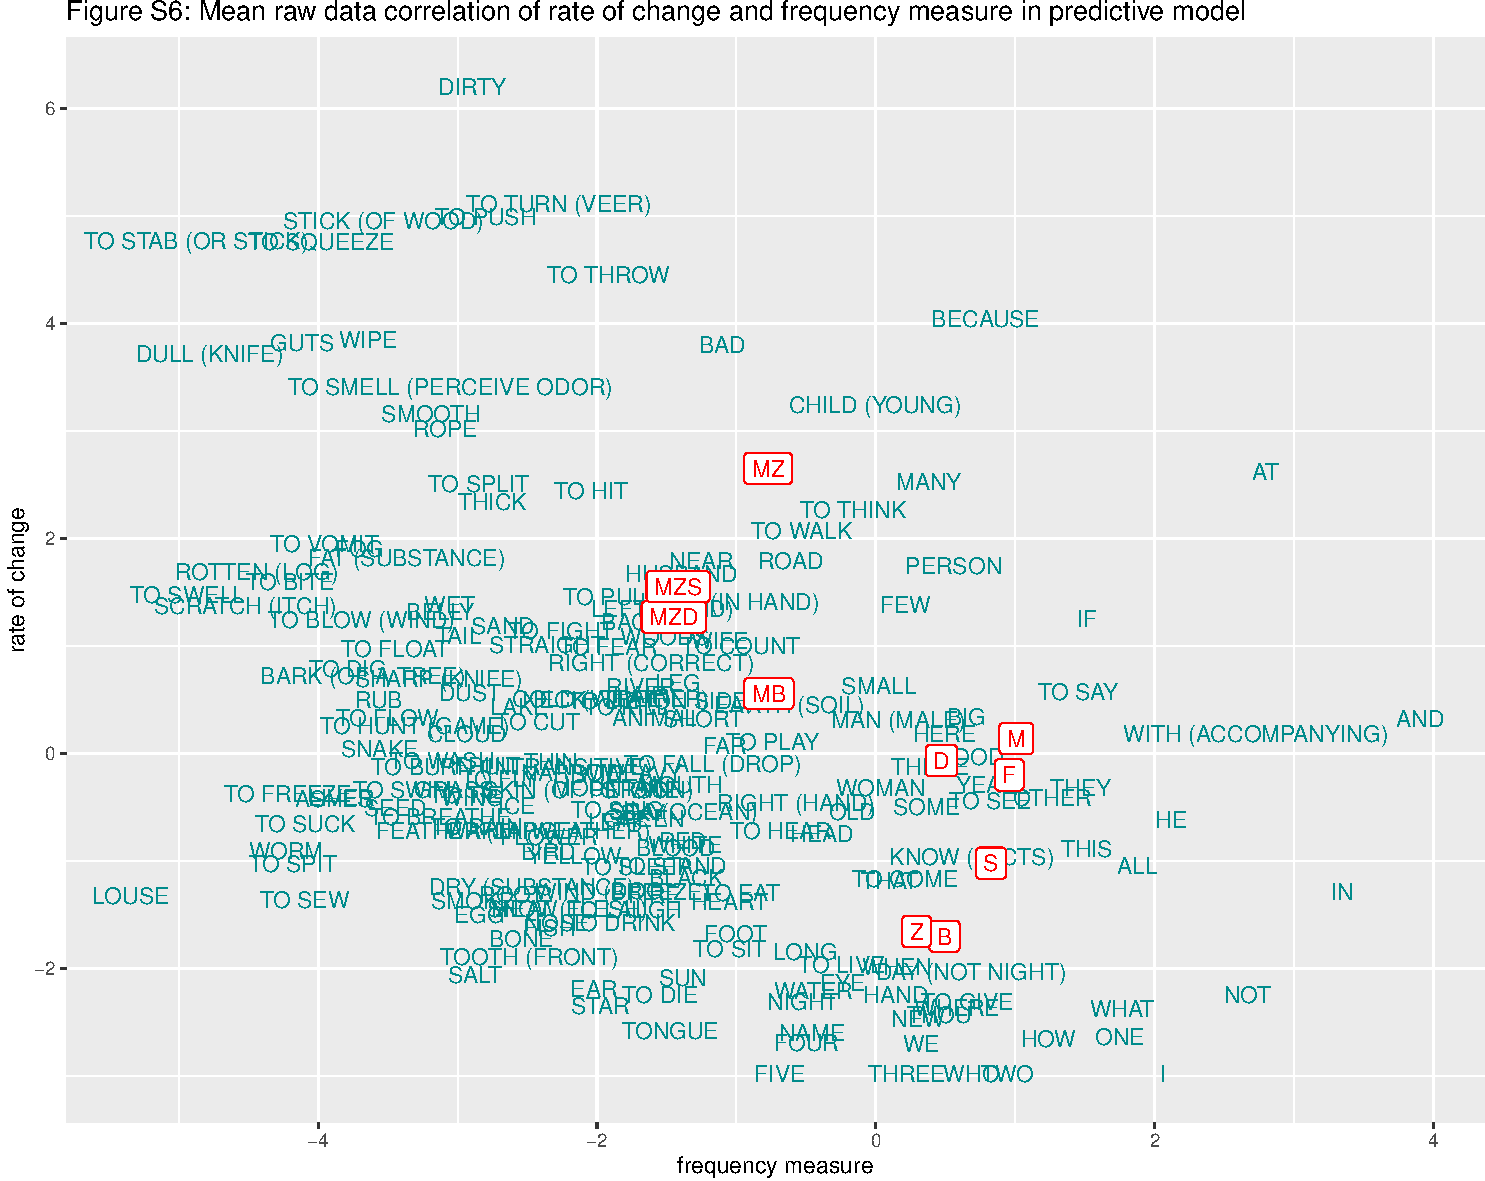
\includegraphics{figures/unnamed-chunk-10-1.pdf}

Table S18: Summary of fixed effects for control model 1b

Estimate

Std. Error

t value

(Intercept)

0.64

0.31

2.03

frequency.measure

-0.58

0.07

-8.72

word.length

-0.10

0.06

-1.76

\subsection{Predictive model: rate of change and frequency of
use}\label{predictive-model-rate-of-change-and-frequency-of-use}

We use the word intercepts from the control model as measures of
frequency of use for kin terms, and centralised log frequency per
million for the Swadesh terms. We restrict the dataset to languages for
which we have kin term data.

Table S19: Summary of fixed effects for predictive model

Estimate

Std. Error

t value

(Intercept)

0.12

0.12

1.01

frequency.measure

-0.44

0.08

-5.26

word.typeswadesh.word

-0.54

0.18

-2.91

frequency.measure:word.typeswadesh.word

0.18

0.09

2.02

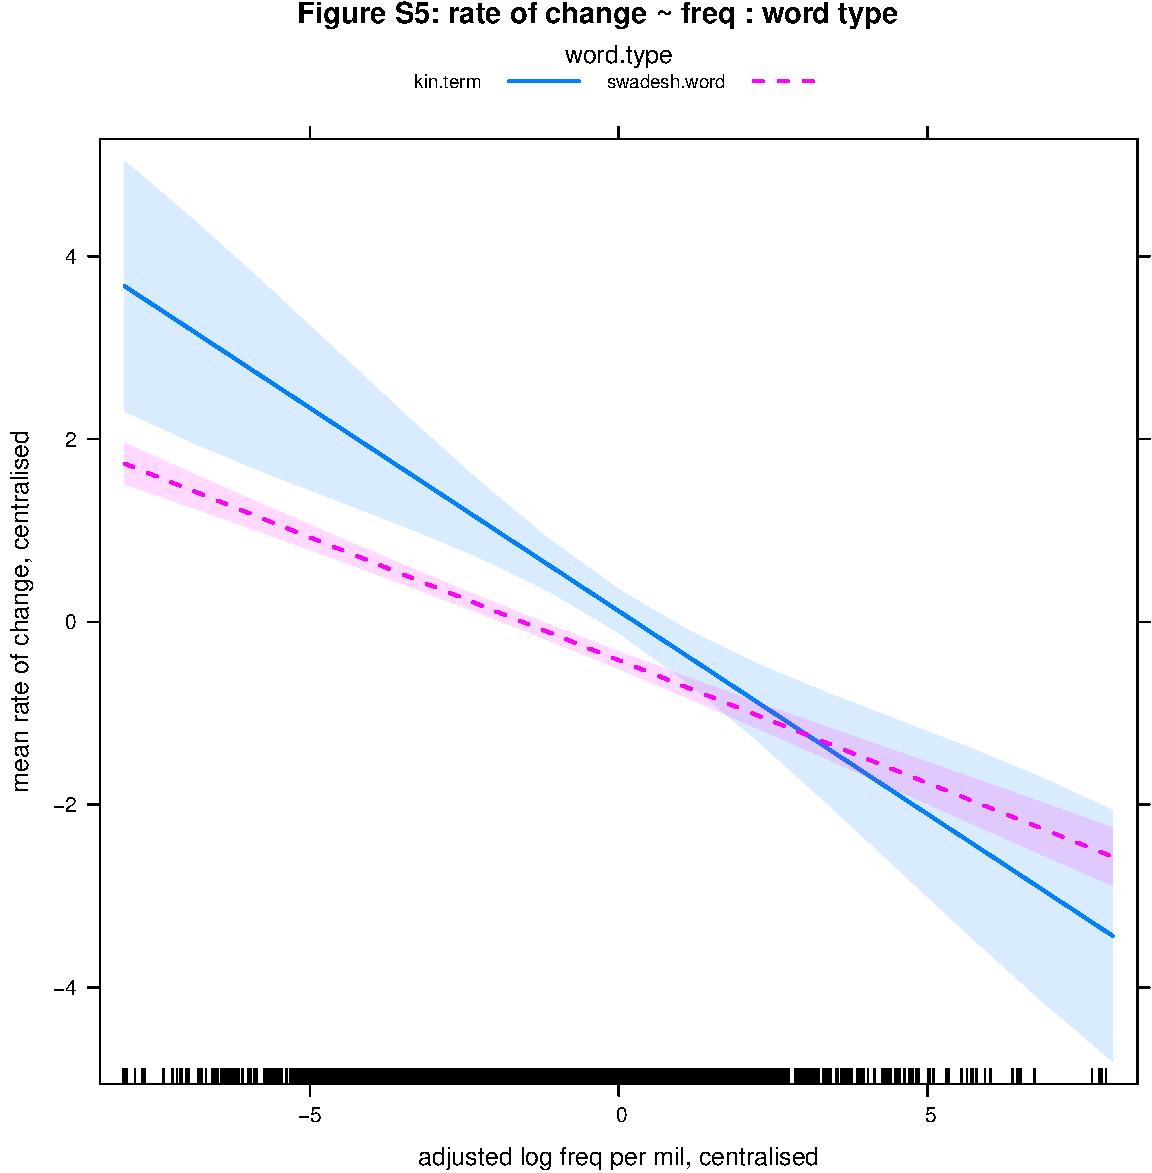
\includegraphics{figures/unnamed-chunk-13-1.pdf}

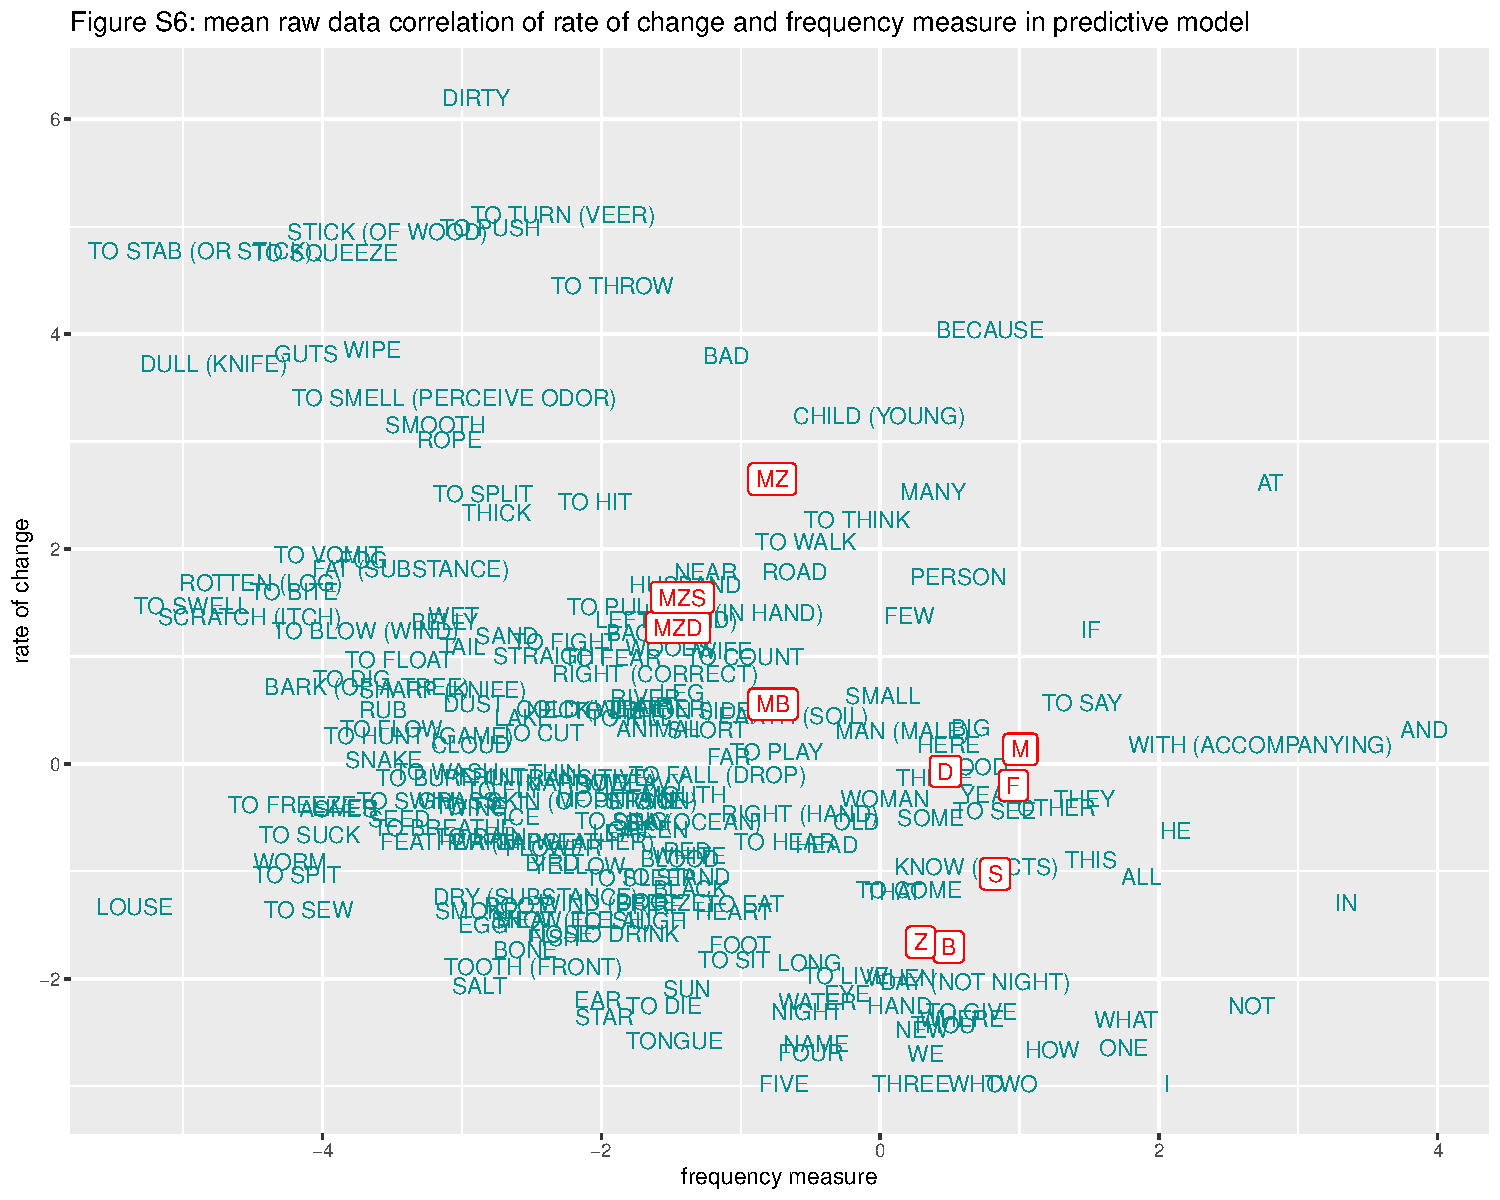
\includegraphics{figures/unnamed-chunk-14-1.pdf}

\section*{References}\label{references}
\addcontentsline{toc}{section}{References}

\hypertarget{refs}{}
\hypertarget{ref-baayen1993celex}{}
Baayen, R Harald, Richard Piepenbrock, and Rijn van H. 1993. ``The
\(\{\)Celex\(\}\) Lexical Data Base on \(\{\)Cd-Rom\(\}\).'' Linguistic
Data Consortium.

\hypertarget{ref-benevsova2013oral2013}{}
Benešová, L, M Kren, and M Waclawicová. 2013. ``ORAL2013:
Reprezentativni Korpus Neformálni Mluvené Ceštiny {[}Oral2013: A
Representative Corpus of Informal Spoken Czech{]}.'' \emph{Ustav
ˇCeského Národniho Korpusu FF UK, Praha}.

\hypertarget{ref-bouckaert_mapping_2012}{}
Bouckaert, Remco, Philippe Lemey, Michael Dunn, Simon J. Greenhill,
Alexander V. Alekseyenko, Alexei J. Drummond, Russell D. Gray, Marc A.
Suchard, and Quentin D. Atkinson. 2012. ``Mapping the Origins and
Expansion of the Indo-European Language Family.'' \emph{Science} 337
(6097): 957--60.
doi:\href{https://doi.org/10.1126/science.1219669}{10.1126/science.1219669}.

\hypertarget{ref-buck}{}
Buck, Carl Darling. 2008. \emph{A Dictionary of Selected Synonyms in the
Principal Indo-European Languages}. University of Chicago Press.

\hypertarget{ref-craveiro2012time}{}
Craveiro, Olga, Joaquim Macedo, and Henrique Madeira. 2012. ``It Is the
Time for Portuguese Texts!'' In \emph{International Conference on
Computational Processing of the Portuguese Language}, 106--12. Springer.

\hypertarget{ref-ek1997czech}{}
Čermák, Franti ek. 1997. ``Czech National Corpus: A Case in Many
Contexts.'' \emph{International Journal of Corpus Linguistics} 2 (2).
John Benjamins Publishing Company: 181--97.

\hypertarget{ref-favretti2002coris}{}
Favretti, R Rossini, Fabio Tamburini, and Cristiana De Santis. 2002.
``CORIS/Codis: A Corpus of Written Italian Based on a Defined and a
Dynamic Model.'' \emph{A Rainbow of Corpora: Corpus Linguistics and the
Languages of the World}, 27--38.

\hypertarget{ref-gelman1992inference}{}
Gelman, Andrew, and Donald B Rubin. 1992. ``Inference from Iterative
Simulation Using Multiple Sequences.'' \emph{Statistical Science}.
JSTOR, 457--72.

\hypertarget{ref-gustafson2006manual}{}
Gustafson-Capková, Sofia, and Britt Hartmann. 2006. ``Manual of the
Stockholm Umeå Corpus Version 2.0.'' \emph{Stockholm University}.

\hypertarget{ref-ion2012rombac}{}
Ion, Radu, Elena Irimia, Dan Stefanescu, and Dan Tufis. 2012. ``ROMBAC:
The Romanian Balanced Annotated Corpus.'' In \emph{LREC}, 339--44.
Citeseer.

\hypertarget{ref-kilgarriff2014sketch}{}
Kilgarriff, Adam, Vít Baisa, Jan Bušta, Miloš Jakubíček, Vojtěch Kovář,
Jan Michelfeit, Pavel Rychly, and Vít Suchomel. 2014. ``The Sketch
Engine: Ten Years on.'' \emph{Lexicography} 1 (1). Springer: 7--36.

\hypertarget{ref-koeva2010bulgarian}{}
Koeva, Svetla, Diana Blagoeva, and Siya Kolkovska. 2010. ``Bulgarian
National Corpus Project.'' \emph{Politics} 207: 2--2.

\hypertarget{ref-kruyt199738}{}
Kruyt, MWF, and others. 1997. ``A 38 Million Words Dutch Text Corpus and
Its Users.'' \emph{Lexikos} 7 (7). Bureau of the WAT: 229--44.

\hypertarget{ref-list_lingpy._2018}{}
List, Johann-Mattis, Simon J. Greenhill, and Robert Forkel. 2018.
``LingPy. A Python Library for Historical Linguistics.''
\url{http://lingpy.org}.

\hypertarget{ref-lyashevskaya2009chastotnyj}{}
Lyashevskaya, ON, and SA Sharov. 2009. ``Chastotnyj Slovar'sovremennogo
Russkogo Iazyka (Na Materialakh Natsionalnogo Korpusa Russkogo
Iazyka){[}Frequency Dictionary of Modern Russian Based on the Russian
National Corpus{]}.'' \emph{Moscow: Azbukovnik}.

\hypertarget{ref-moreno2005spanish}{}
Moreno-Sandoval, Antonio, Gillermo De la Madrid, Manuel Alcántara, Ana
Gonzalez, José Maria Guirao, and Raúl De la Torre. 2005. ``The Spanish
Corpus.'' \emph{C-ORAL-ROM: Integrated Reference Corpora for Spoken
Romance Languages, Amsterdam: John Benjamins Publishing Company},
135--61.

\hypertarget{ref-morozova2015albanian}{}
Morozova М, Rusakov А. 2015. ``Albanian National Corpus: Composition,
Text Processing and Corpus-Oriented Grammar Development.'' \emph{Sprache
Und Kultur Der Albaner. Zeitliche Und Räumliche Dimensionen.} 5:
270--308.

\hypertarget{ref-new2001base}{}
New, Boris, Christophe Pallier, Ludovic Ferrand, and Rafael Matos. 2001.
``Une Base de Données Lexicales Du Français Contemporain Sur Internet:
LEXIQUE™//a Lexical Database for Contemporary French: LEXIQUE™.''
\emph{L'année Psychologique} 101 (3). Persée-Portail des revues
scientifiques en SHS: 447--62.

\hypertarget{ref-pagel_deep_2018}{}
Pagel, Mark, and Andrew Meade. 2018. ``The Deep History of the Number
Words.'' \emph{Phil. Trans. R. Soc. B} 373 (1740): 20160517.
doi:\href{https://doi.org/10.1098/rstb.2016.0517}{10.1098/rstb.2016.0517}.

\hypertarget{ref-przepiorkowski2010recent}{}
Przepiórkowski, Adam, Rafal L Górski, Marek Lazinski, and Piotr Pezik.
2010. ``Recent Developments in the National Corpus of Polish.'' In
\emph{LREC}.

\hypertarget{ref-przepiorkowski2008towards}{}
Przepiórkowski, Adam, Rafal L Górski, Barbara Lewandowska-Tomaszyk, and
Marek Lazinski. 2008. ``Towards the National Corpus of Polish.'' In
\emph{LREC}.

\hypertarget{ref-ulfarsdottir2017lexicography}{}
Úlfarsdóttir, Thórdís, and Kristín Bjarnadóttir. 2017. ``The
Lexicography of Icelandic.'' \emph{International Handbook of Modern
Lexis and Lexicography}. Springer, 1--12.

\hypertarget{ref-van2007over}{}
Van Eerten, Laura. 2007. ``Over Het Corpus Gesproken Nederlands.''
\emph{Nederlandse Taalkunde} 12 (3): 194--215.


\end{document}
